\chapter{码中一窥C++}


凡是语言,都一定有着自己的规则。而不同于英语、汉语这种自然语言,作为计算机所能识别的语言,它是需要在严格约束下避免二义性的,所以说我们将学到的C++语言,是一门语法规则非常严格,但又“灵活多变”的语言。

所谓非常严格,是指C++中不允许出现歧义,这种没有歧义的文法是经过严格的文法规则的限制、和一些约定来约束的。所以,如果在你的代码中出现了自己都会觉得有歧义的地方,往往就是程序中容易出错的地方。

而所谓灵活多变,就是指在掌握C++严格的语法之后,可以写出无穷无尽充满创意的程序。从黑框(控制台程序),到带有图形界面(GUI)的程序,再到游戏,都可以利用C++的语法加上你脑中的算法搞定!而所有的这些灵活多变的内容,都是在严格的文法约束下实现的。所以说C++语言,是一门语法规则非常严格,但又灵活多变的语言!

C++是一门高级语言,所谓高级语言正如你们在前面章节中看到的,是不同于机器语言、汇编语言;能更加贴近人类思维的一门语言。C++是在C语言的基础上,增加了例如面向对象编程等诸多特性的程序设计语言。在程序设计竞赛中被广泛采用。

非常不严格地讲:我们常常所说的“C++”,包含了这门语言和一系列的工具。语言顾名思义就不多阐述。而工具实际上包含了很多内容:

我们将C++语言所编写的代码叫做“源代码”。而源代码是不能直接被计算机执行的(回想我们在上一章中讲述的内容)。而是应该利用编译程序,将源代码编译成计算机能够识别的机器代码然后再执行。而执行编译工作的工具就叫做“编译器”。

除此之外,仅仅有C++语言,我们连基本的功能(例如屏幕输出)都实现不了。即便是高级语言,想要与硬件设备交互,一般都需要直接编写一定的机器语言或者汇编语言,所以才能让我们的程序操作硬件:屏幕打印、屏幕输入、文件操作等等。而我们想要通过一己之力实现这些最底层的操作是很困难的。好在C++提供了一组可以被调用的工具。这些工具其实就是别人写好的代码,通过C++语法能够接受的形式所调用,最终辅助我们完成底层调用的功能,让我们的精力能够集中在更重要的算法设计上而不是千篇一律的与底层的通讯上。我们称这种“别人的代码”叫做“库”。就如同仓库一样,我们可以调用仓库中的内容来实现我们的意图。

那么我们的程序是怎么与别人的程序产生关联的呢?这有很多种情况,我只讲述最常见的一种:静态链接。我们的程序在调用库的时候,编译器可以仅仅在相应的位置上做个标记,表明这里的程序是调用了库而不是我自己的。这么做的好处就是可以充分地提高编译效率。因为库中的代码往往经过严格的编写、测试,基本能保证没有问题,所以我们只需要保存该库编译完毕的状态,没有必要在编译自己的程序时还要将别人的库再编译一遍。我们只需要编译自己的程序就可以了。所以我们的程序与库之间是并列关系,而不是包含关系。但是想要让自己的程序能够变成可执行程序,仅仅是这种“做标记”的方法是不可接受的。因为你所需要的库文件在你的电脑上会有,但并不意味着别人的电脑上也会有。再加上可执行程序的复杂原理,我们必须将这些静态库与我们的程序绑定在一起。而将编译完的“目标代码(Object Code)”与库文件链接形成“可执行文件”的工具叫做“链接器”。

也就是说,C++程序设计流程是:
\begin{quote}
	\begin{enumerate}
		\item 编写代码
		\item 编译成目标代码
		\item 链接成可执行文件
	\end{enumerate}
\end{quote}


一般来说,想要实现上面的流程,需要利用操作系统提供的黑框(Linux下的终端、Windows下的控制台),再加上一大堆非常复杂的命令才能实现。编译命令甚至有可能比源代码还要复杂。如果需要对自己的代码进行调试,那可是更加麻烦。所以聪明人们就为懒人发明了又一件工具:集成开发环境(Integrated Development Environment,IDE)。所谓开发环境,可以将其看作是写代码的一个工具。我们可以在这个开发环境中编写代码、代码着色、自动排查错误等。所谓“集成”就是指将“编译器”、“连接器”都集中在IDE中。程序员可以简简单单地点击按钮,就可以实现整套编译链接运行调试等功能。

在ACM/ICPC的比赛中,通常使用的编译器是GCC(GNU Complier Collection)。GCC是一个支持很多种语言的开源的编译器的集合。它可以安装在Windows(不推荐)和Linux等多种操作系统上。而在比赛中普遍使用的是安装了Linux操作系统和GCC编译器的开发环境,并且配置了某些IDE来让学生进行开发。

关于IDE:对于Windows来说,我门推荐使用Dev-C++。对于Linux,我们推荐使用Code-Blocks。

本章的行文基于“CART”步骤,即(C)ode, (A)nalyze, (R)esult, (T)ry。四步。

Code是指展示代码,Analyze是针对代码分析其中的语法元素,Result是根据程序的运行结果来分析程序的逻辑,Try则是举一反三,完成与该代码相关的另一段代码的编写。

\section{Helloworld++}
其实吧,作为一名编程初学者,第一个编写的程序应该就是传说中的“Helloworld”。这个程序意图就是在屏幕上简简单单地打印出一个“Helloworld”的文字。目的是为了表示当前的开发环境没啥问题,可以继续工作了。

但是我觉得一个Helloworld太简单了,各种书籍都把这个例子用烂了,那我在这里就用一个稍微复杂的例子来实现这个“Helloworld”吧!

\subsection{Code}
\lstinputlisting[language=C++,caption=Helloworld++,label=code:helloworld++]{codes/1-1/1-1.cpp}

\subsection{Analyze}
代码\ref{code:helloworld++}是加强版的Helloworld,所以我管它叫做Helloworld++。代码首先通过提示依次输入你的姓名和性别,再根据不同的性别输出不同的“问候语”。对它的部分解读如下:
\begin{quote}
\showremarks
\end{quote}

我们再来逐行精读这段代码。

首先,代码\ref{code:helloworld++}的前两行中使用了“\#include<xxxxx>”。这部分内容叫做“预编译指令\footnote{也叫做预处理指令。}”。所谓预编译,就是指在编译之前要“告诉”编译器的“话”。编译器收到这些指令之后就会按照指令上的内容提前进行一些预处理。

在C++中常见的预处理指令主要有“\#include”、“\#define”等。当然还有一些诸如“\#ifndef”等在本书中不是很常用的预处理指令。

“\#include xxx”用来表明该段程序编译前应该包含哪些其他文件。由于操作系统会将一些常用的操作封装成函数库,并写在某些自带的文件中,所以当我们使用这些函数库的时候,一般都需要通过该命令将其包含。命令中的xxx则是用“<>”或者双引号括起来的文件名。用“<xxx>”则表示这个文件在系统的搜索路径下保存,一般是系统库。而用双引号扩起来的则表示这个文件跟当前程序代码文件存放在同一个文件夹。

而“\#define A B”则是表示强行将B替换成A。也就是说在以后的代码中凡是出现过“B”的地方都将会无条件地被替换成“A”。在C语言\footnote{C++的前身,C++就是对C语言扩展而成的语言}时代,常常用这种方法来避免一些硬编码\footnote{即“直接将常数值分布在程序的各处”,这种硬编码导致的程序冗余性会让代码修改起来非常困难。}。例如有一个运算式频繁使用了PI=3.14这个数值。但是突然想要让PI=3.1415。这时候需要把所有的3.14替换成3.1415。但如果很早之前我们的程序就是用PI来表示这个值,在此时也就只需要将“\#define PI 3.14”改成“\#define PI 3.1415”即可。

由于“\#define”是在“编译前”执行,所以它带来的开销不会在程序运行时体现出来,而且还能进行很多技巧性的操作。但是由于这种“技巧性”的操作稍有不慎就可能产生很麻烦的后果,所以不建议初学者滥用这种方法。而它所提供的功能可以通过类似但更加安全的方法实现。

代码\ref{code:helloworld++}的第三行用来“使用命名空间”。所谓命名空间,是一种C++对多文件多函数的组织工具。我们常常把功能相近的函数库放在一个模块中,为这个模块可以取一个好记的名字。当以后使用这些函数库时,就可以使用using namespace xxx; 这样的语句来使用。

在代码下面的诸如“cin”、“cout”、“endl”等内容,以及以后大家将会接触到的一些函数库都需要“std”命名空间,大家记住在每次编写代码时都写上这一句就好了。有关命名空间的详细主题已经超过本书“速成”的要旨,就不多介绍了。

程序的第五行是定义了主函数。所谓函数,暂时可以理解为对一组操作的包装\footnote{术语叫做“封装”}。而主函数则是整个程序的入口。可执行文件被打开后,操作系统将会从主函数开始依次执行。在主函数中又调用了各种各样其他的程序,以此来完成整个运行逻辑。

之所以称之为主函数是因为它的结构。int main()表明这是一个返回int类型\footnote{什么叫做“返回int类型”,我们稍后再谈}的函数,而函数名“main”则表明了这个函数是一个主函数。后面紧跟着一个大括号。主函数内部的东西都写在了这个大括号中。

一般来说,大括号表示一段语句,而其中的语句隶属于这个大括号,所以在大括号中的代码应该比外面的代码多缩进一截。这么做对编译器没有任何影响,只是为了让代码层次感明确、易读。所以希望大家都遵守这个惯例!

在大括号中的内容就是系统会执行的代码。第七行的内容称为注释。注释就是一种会自动被编译器所屏蔽的“非代码”。注释能够辅助程序员解释代码功能,增加代码可读性。同时由于“被注释后会被编译器忽略”的特性,使得注释可以用来“临时屏蔽”一些代码。

在C++中添加注释有两种方法。一种是行注释:“//”——两条正斜杠后面的内容都是注释。还有一种是块注释:“/*”到“*/”中间的所有内容,无论经过多少行,都会被看做是注释。正如同代码的第7、10、13行。

在代码的第8行,声明了一个常量。此处的常量与数学意义上的常量非常类似。常量的定义通常由两部分。

一部分是定义部分,形如“const int trunk\_size”。其中“const”是定义常量的关键字\footnote{一般与“保留字”等价。他们是一种特殊的单词,这些单词不能作为常量、变量名等用户自定义的内容。因为它们本身已经被C++编译器赋予了神圣的意义。}。“int”表示这个常量的类型是“整型”。关于数据类型将会在后面介绍。“trunk\_size”就是变量名咯,是这个常量的名字。

另一部分是赋值部分,形如“trunk\_size=100”。这部分内容就是指令常量“trunk\_size”等于常量值“100”。(跟我们学过的数学完全一样是吧!)

既然名叫常量,则就说明这个量一经定义不许再在程序中改变。所以常量的定义部分和赋值部分是合在一起的,形如第8行代码。此之于“变量”来说是略有不同的,我们将稍后再说。

在第11行和14、15行有两条非常相似的语句。这就是传说中的变量定义。其实变量定义跟常量定义非常相似,反倒是常量定义麻烦了一些——变量定义不需要const修饰。在11行,定义了变量,并且直接在等号右边赋值。第14行则是先定义变量,再在第15行赋值。

变量定义部分的“char *”表示了这是个“字符指针类型\footnote{指针,即“保存内存地址”的变量,该主题将会在后面谈到}”。“name”和“sex\_str”是变量名。而等号后面的赋值部分,实际上是在进行“在堆中申请一段连续存储空间”的操作。上面这堆文字具体的意义我们后面会详细提到,目前你只需要知道这就是声明变量的一种方法就好了!

在第17,18行,有一种“cout<<xxxx<<endl;”的格式。其中cout是输出流对象。也就是说需要输出的时候就靠它。而在第19行的cin则是代表输入流对象。这两种对象对应着不同的符号进行控制。如果说这种大于号和小于号类似于箭头,则可以将“cout”和“cin”分别看作是屏幕和键盘。数据从箭头起点处流向目标。而且cout和cin必须要写在开头。于是就有了例子中的样式:第17行的“Who are you”作为数据,被传送到了cout这个“屏幕”。然后又将“endl”这个换行符传递给了cout。在第19行则表示将键盘的内容输出到“name”这个变量中。

代码的第17-23行都是在进行输出和输入。而在24行到28行则是一种特殊的结构——选择结构。

所谓选择结构,就是指根据某个条件进行选择。如果这个条件成立则做事情A,如果另一个条件成立则做事情B,以此类推,直到什么都不成立的时候,则做另一个事情。

这五行代码是选择结构中的if语句。形式大约是:
\begin{quote}
if(<事件A>)\{

	\qquad 若A事件成立则执行此块
	
\}else if(<事件B>)\{

	\qquad 若B事件成立则执行此块
	
\}else\{

	\qquad 若都不满足则执行此块
	
\}
\end{quote}

值得注意的是在第24行的“strcmp("boy",sex\_str)”。这是一个系统库“<cstring>”中的函数“strcmp(strA,strB)”。这个函数的功能是比较字符串。若strA与strB的内容完全相等,则它的值等于0。在这个函数调用前的感叹号是“取反”符号,功能就是让1变0、0变1。所以这段代码的逻辑就是:如果sex\_str等于“boy”,则执行第25行。否则执行27行。

在第29行,“return 0”表示这个函数返回“0”。由于这个函数是主函数,则它的返回值将会被操作系统所接收\footnote{有关函数和返回值的相关主题将会在后面介绍}。

至此我们便大致分析了这个“Helloworld++”程序。接下来我们执行以下看看结果!

\subsection{Result}

根据程序逻辑,这段代码执行时要先输入一个名字,然后输入boy或者girl,屏幕则会根据这些不同的输入打印出不同的响应文字。
\\[\intextsep] 
  \begin{minipage}{\textwidth} 
    \centering 
    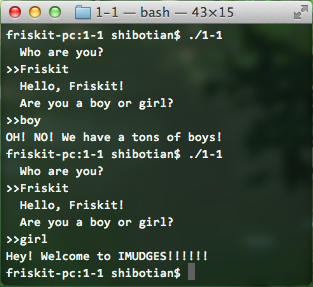
\includegraphics{codes/1-1/result.png}
    \figcaption{Helloworld++} 
    \label{fig:code-1-1-result} 
  \end{minipage} 
\\[\intextsep] 

我们再来分析一下这个程序的运行逻辑。
\begin{quote}
	\begin{description}
		\item[步骤1>>]在程序的1-2行,通过预编译指令,包含了两个函数库文件。
		\item[步骤2>>]在程序的第5行找到程序的入口、主函数。
		\item[步骤3>>]在程序的第8~15行定义了一系列常量和变量。
		\item[步骤4>>]在程序17~18行输出提示信息,让用户输入名字。
		\item[步骤5>>]等待用户输入名字,并将输入内容存储至变量“name”。
		\item[步骤6>>]再提示用户输入性别。
		\item[步骤7>>]等待用户输入性别,是“boy”或者“girl”。并且将输入内容存储至变量sex\_str。
		\item[步骤8>>]判断sex\_str里的内容。
		\item[步骤9>>]如果内容是“boy”则执行第25行的输出。
		\item[步骤10>>]如果内容不是“boy”则执行第27行的输出。
		\item[步骤11>>]主函数返回,程序结束。
	\end{description}
\end{quote}

至此就是这个程序的运行流程。

我们再来小结一下上面的程序所遇到的内容!希望大家在看到这些名词之前能努力回忆一下它们的具体含义。然后再看后面的解释内容!

\begin{description}
	\item[预编译指令]被编译器在编译前执行的命令。包括“\#include”、“\#define”等等。
	\item[命名空间]命名空间是C++用来高效地组织各种代码的方法。通常我们使用的命名空间是“std”。用法是:using namespace std;
	\item[主函数]整个程序运行的入口。它的返回值将会被操作系统所接收,你可以通过返回值告诉操作系统这个程序结束执行时的状态。例如0表示正常,-1表示错误。
	\item[变量]变量就如同数学中的概念一样,是一种可以变化的量。变量就是内存中固定大小的一块存储空间,其大小由其类型决定。变量使用前需要预先定义!
	\item[常量]常量是一种一经定义就不能改变的量,也正是因为这个特性,它必须在定义的时候立刻赋值。将一般不会改变的数存储成常量而不是变量,一来能防止不小心地修改这些值,另一方面能够通过系统的内存管理机制得到优化。
	\item[标准输入输出]即“cout”和“cin”。就是一种用来控制“输出到屏幕”和“从键盘读取”的工具。大于号或者小于号表示输出方向。将“cout”看作是屏幕、将“cin”看作是键盘,将会比较容易加深记忆。
	\item[if语句]它就是一种选择结构的语句。就如同数学中的分段函数一样,根据不同的条件进行不同的操作。大家再回忆一下它的形式。
	\item[语句]语句就是C++程序中的基本组成单位。变量定义可以使一个语句、赋值操作可以是语句、函数调用可以是语句,还有一些程序控制语句(例如if语句等)。总之,我们的程序是由一个个语句组成的。在语句之中可以嵌套其他语句。
	\item[关于分号]一般来说,除了预编译指令以外,我们需要在每一个语句完成之后加上分号。
\end{description}

在这一节中,大家了解到了一个完整的不算大也不算小的C++程序的样子。我们今后所编写的代码也基本都长这个样子,区别就是主函数里头的东西可能更丰富、算法更高深等等。但是这个整体的框架是万变不离其宗的。所以希望大家能够根据上面的例子“改造”出自己的代码来。

\subsection{Try}

在了解完上面的例子,我们可以用类似的代码“创作”出一些自己的程序!

\begin{description}
	\item[Try 1]制作一个程序,在屏幕上输出一行“Hello World!”。
	\item[Try 2]制作一个加法运算器,根据提示分别输入加数和被加数,并且输出两者相加的结果。
	\item[Try 3]制作一个程序:用户输入数字1-7,输出汉语“星期x”,(使用连续的if-else if语句)
\end{description}

\section{使用变量与数据类型}
我们在前面曾经讲过,现在的计算机都是一种“存储计算模型”。“存储”在程序中的体现就是“变量”。变量其实就是在程序运行时用来存储数据的容器。它的物理结构就是内存中的某一块固定大小的区域。尽管都是用“0”、“1”将内存区域填满,但不同类型的变量所占用内存单元的数量会有所不同,也会导致这种类型所表示的数据范围的不同。同时,一般的数据类型还有“有符号”和“无符号”的区别。这是由于计算机利用数据单元中的1位来表示正负,所以即便是能够表示数字的数量相同,但能表示的范围仍有所区别。

在C++中有一些内置的基本数据类型,用户也可以定义自己的数据类型。不同的数据类型以不同的排布方式放置在内存中。数据相同的内存单元,用“不同类型的角度”来看都有不同的取值。常见的基本内置数据类型如下:

\begin{center}
	\begin{tabular}{|c|c|c|c|}
		\hline
			数据类型 & 长度 & 能表示的数据范围\\
		\hline
			char & 1 & $-128 \sim 127$				\\
			short & 2 & $-32768 \sim 32767$			\\
			unsigned short & 2	 & $0 \sim 65535$\\
			int & 4 & $-2147483648 \sim 2147483647$	\\
			unsigned int & 4 & $0 \sim 4294967295$ \\
			long & 8\footnote{在32位计算机上长度可能为4字节,功能和取值范围与int完全一致} & $-9223372036854775808 \sim 9223372036854775807$	\\
			unsigned long & 8 & $0 \sim 18446744073709551615$ \\
			float & 4 & $-3.4\times10^{-38} \sim 3.4\times10^{38} $ \\
			double & 8 & $-1.7\times10^{-308} \sim 1.7\times10^{308} $\\
		\hline
	\end{tabular}
\end{center}

了解了上述的数据类型之后,让我们来看看这一节的代码吧。

\subsection{Code}

\lstinputlisting[language=C++,caption=数据类型,label=code:Datatype]{codes/1-2/1-2.cpp}


\subsection{Analyze}

\subsection{Result}

\subsection{Try}